% Steering Taxonomy paper -- ACL/EMNLP format.
%
% Target venue: ACL Findings (long paper, 8 pages + unlimited refs/limits).
% Requires the official ACL style file (acl.sty + acl_natbib.bst).
% These are committed to acl_style/ for convenience; the official source
% is https://github.com/acl-org/acl-style-files
%
% Compile with `pdflatex` -> `bibtex` -> `pdflatex` x 2.
% Add `TEXINPUTS=./acl_style:` and `BSTINPUTS=./acl_style:` to your env if
% the .sty / .bst are not on the default LaTeX path.
%
% Use `[review]` for anonymized submission, no option for camera-ready.

\documentclass[11pt]{article}

\usepackage{acl}
\usepackage[T1]{fontenc}
\usepackage[utf8]{inputenc}
\usepackage{amsmath,amssymb}
\usepackage{booktabs}
\usepackage{graphicx}
\usepackage{url}
\usepackage{xcolor}

\title{When Activation Steering Works:\\
       A Geometric Predictor Across 12 Tasks and Two Model Families}

\author{Suleman Imdad \\
  Johns Hopkins University \\
  \texttt{suleman.imdad@me.com}}

\begin{document}
\maketitle

% ===========================================================================
\begin{abstract}
% ===========================================================================
Activation steering produces striking results on some tasks (refusal,
sentiment) and quietly fails on others. We ask: \emph{when} does it
work? We run a unified, controlled protocol across 12 tasks and
characterize each task's contrastive direction along two axes: a
\textbf{geometric} axis (split-half cosine stability and per-pair
angular variance of the contrastive direction) and an \textbf{empirical}
axis ($\Delta$ vs.~baseline and $\Delta$ vs.~a random-direction control).
The data refutes the naive hypothesis that a low per-pair variance
signals a stable, steerable axis: near-zero per-pair variance instead
correlates with whether the contrast collapses onto a cosmetic
framing word that the model does not condition on. The empirically
derived rule---\emph{split-half cosine $\geq 0.7$ AND per-pair
variance $\geq 0.3$ implies steering succeeds}---achieves 9 of 12
(75\%) task-level accuracy on Llama-3.2-3B-Instruct, and the
three exceptions identify a third axis the geometry cannot see alone:
\emph{contrast asymmetry} (presence-vs-absence of a structural prefix
produces strong steering despite near-zero per-pair variance). The
augmented three-axis rule generalizes \emph{out-of-sample}: pooled
leave-one-task-out across 48 (model, task) pairs from four models
(Llama-3.2-\{1B, 3B\}, Qwen2.5-\{3B, 7B\}) gives 79.2\% accuracy,
with cross-model validation (train on three models, test on the
never-seen fourth) yielding 75--83\% per held-out model and
near-identical chosen thresholds on every split. Geometric features
themselves agree across families to within $\pm 0.05$ on all 12
tasks---the $(\text{cos}, \text{var})$ signature is a property of the
contrast, not the model. The conventional behavioral
vs.~content-specific task taxonomy is not predictive in our data:
rag\_distractor (content-specific) steers as hard as refusal
(behavioral), and honesty (behavioral) does not steer at all.
\end{abstract}

% ===========================================================================
\section{Introduction}
% ===========================================================================

Activation steering---adding (or projecting out) a precomputed
direction in a language model's residual stream at inference
time---has become a popular tool for behavioral
control~\citep{turner2023activation,zou2023representation,
li2023iti,rimsky2023steering,arditi2024refusal,yang2026contextfocus}.
Reported effects span the dramatic (40\,pp+ on refusal
suppression~\citep{arditi2024refusal}; 35\,pp+ on
context-faithfulness~\citep{yang2026contextfocus}) to nearly null.
The literature documents the successes; the failures rarely get
their own paper. As a result, we lack a principled answer to a
basic question: \emph{given a candidate behavior, can we predict in
advance whether activation steering will move it?}

We answer ``mostly yes, with one twist'' using a diagnostic computed
from the contrastive pair set alone, before any held-out evaluation:

\begin{quote}
\textbf{High split-half cosine AND high per-pair variance predict
steering success.} A direction whose mean is stable across pair
subsamples (high cosine) \emph{and} whose individual pair-directions
span a wide angular range (high variance) is capturing a real
semantic axis amid varied content; ablating it moves the metric on a
held-out evaluation. If the cosine is low, the mean direction is
essentially noise. If the variance is near zero, the contrast has
typically collapsed onto a single token-level feature---usually
cosmetic and behaviorally inert.
\end{quote}

The one twist: a small minority of tasks have near-zero variance
\emph{and} steer strongly. They all share a structural-asymmetry
property in their contrast (positive prompts include a system
prefix or context block; negative prompts omit it entirely). The
geometric axes alone cannot detect this case.

\paragraph{Contributions.}
\begin{itemize}
\item A \textbf{unified protocol} that produces a uniform per-task
report combining geometric characterization (split-half cosine,
per-pair variance) with empirical characterization (baseline,
steered, random-direction control) for any contrastive
direction.
\item A \textbf{12-task corpus} spanning canonical behavioral targets
(refusal, honesty, sycophancy, sentiment, truthfulness),
content-specific targets (rag\_distractor, fact\_override,
topic\_suppression), and borderline cases (context\_faithfulness,
persona, politeness, hallucination\_grounding).
\item An \textbf{empirically derived predictive rule} (split-half
cosine $\geq 0.7$ AND per-pair variance $\geq 0.3$ $\Rightarrow$
steering succeeds) that achieves 9 of 12 (75\%) accuracy on
Llama-3.2-3B-Instruct with a wide threshold plateau. We characterize
the three exceptions and identify the additional structural feature
(contrast asymmetry) needed to classify them.
\item \textbf{Out-of-sample validation.} Pooled leave-one-task-out
across 48 (model, task) pairs from Llama-3.2-\{1B, 3B\} and
Qwen2.5-\{3B, 7B\} gives \textbf{79.2\% accuracy} for the augmented
three-axis rule; cross-model CV (train on three models, test on the
fourth) yields 75--83\% on every held-out model with near-identical
chosen thresholds. The geometry-only rule's LOO drops to 58\%---
the asymmetry feature is what closes the gap.
\item \textbf{Probe baseline shows linear separability $\neq$
behavioral conditioning.} A logistic-regression probe trained to
discriminate the contrast pairs saturates at $\geq 0.99$ on $7/12$
tasks regardless of whether ablation moves the metric;
$r(\text{probe acc}, |\Delta_{\text{rand}}|) = -0.176$ while
$r(\bar{\cos}\cdot\sigma, |\Delta_{\text{rand}}|) = +0.436$.
Steering predicts behavior change; probes predict only
separability.
\item \textbf{Mechanism via Gemma-Scope SAE.} Per-task directions
on Gemma-2-9B-Instruct layer 9 decompose over the SAE feature
dictionary at $r(\text{n features}, \sigma) = +0.75$: structural-
asymmetry tasks collapse onto $\sim$220 features dominated by a
single one (peak coef $\sim$0.65); high-$\sigma$ tasks spread
across 1900--3900 features.
\item A demonstration that the conventional behavioral
vs.~content-specific task taxonomy is \emph{not} predictive of
steering: a content-specific task (rag\_distractor) steers as
cleanly as refusal, while a canonical behavioral target (honesty)
does not steer at all.
\item Open-source code, task corpus, and per-task reports.
\end{itemize}

% ===========================================================================
\section{Related Work}
% ===========================================================================

\paragraph{Activation steering and representation engineering.}
\citet{turner2023activation} introduce activation addition.
\citet{zou2023representation} formalize representation engineering
with framing-pair contrasts. \citet{li2023iti} introduce
Inference-Time Intervention for truthfulness on TruthfulQA.
\citet{rimsky2023steering} demonstrate Contrastive Activation
Addition across many behavioral targets in Llama-2.
\citet{arditi2024refusal} show that refusal in safety-tuned models
is mediated by a single direction discoverable from harmful vs.
harmless prompts. \citet{yang2026contextfocus} apply CAA-style
intervention to context-faithfulness on ConFiQA.

\paragraph{Predicting when steering works.}
A handful of studies report negative or mixed results on activation
steering, often as side observations within larger interpretability
projects. To our knowledge no prior work proposes a pre-evaluation
diagnostic computed from the contrastive pair set alone, validates it
across a broad task corpus, and reports cross-family generalization.

\paragraph{Stability measures.}
Split-half reliability is a standard measure in psychometrics and
cognitive neuroscience and has been used in NLP probing work as a
diagnostic for whether a probed representation reflects a stable
underlying feature. We adapt it to the contrastive-direction setting
as a \emph{pre-evaluation} diagnostic and pair it with per-pair
angular variance to disambiguate stable-but-collapsed contrasts from
stable-and-content-spanning ones.

\paragraph{Linear representation hypothesis.}
Under
LRH~\citep{mikolov2013linguistic,park2023linear,elhage2022superposition},
each per-pair direction decomposes as
$d_i = \alpha_i v + \varepsilon_i$ with $v$ the latent target axis
and $\varepsilon_i$ orthogonal content residual. Two regimes yield
high split-half cosine: (i) \emph{genuine axis}, $\alpha_i$ roughly
constant and $\|\varepsilon_i\|$ large, so $\bar{d} \!\to\! v$ and
$\sigma$ is large; (ii) \emph{collapsed token feature}, every $d_i$
dominated by a shared surface artifact, $\|\varepsilon_i\| \!\to\!
0$, $\sigma \!\approx\! 0$. Only (i) yields the diverse-content
signature the rule predicts as steerable, because the model
conditions on $v$ but not on the surface artifact. Structural
asymmetry is a third regime: the model conditions on a prefix
feature (system or persona), so even $\sigma \!\approx\! 0$
directions can hit a real conditioning subspace.

% ===========================================================================
\section{Protocol}
% ===========================================================================

A steering task in our corpus exposes:
\begin{enumerate}
\item A set of contrastive pairs
$\{(x_i^+, x_i^-)\}_{i=1}^N$---two prompts that differ along the
target behavioral axis.
\item A held-out evaluation set
$\{(p_j, t_j)\}_{j=1}^M$ with a scoring function
$s(\text{completion}, t_j) \in [0, 1]$.
\end{enumerate}

\paragraph{Direction extraction.}
For each pair $i$, we run a forward pass on $x_i^+$ and $x_i^-$,
take the mean-pooled hidden states at the target layer $\ell$, and
form the per-pair direction
$d_i = h(x_i^+; \ell) - h(x_i^-; \ell) \in \mathbb{R}^{d_{\text{model}}}$.
The mean (CAA) direction is $\bar d = \tfrac{1}{N}\sum_i d_i$,
unit-normalized.

\paragraph{Geometric characterization.}
\begin{itemize}
\item \textbf{Split-half cosine.} We randomly split the $N$ pairs
into two halves, compute the mean direction within each half, and
take the cosine similarity between them. We repeat this 20 times
and report the mean ($\bar{\cos}$) and standard deviation.
A high value means the mean direction is robust to which half of
the pairs are used to compute it.
\item \textbf{Per-pair variance.}
$\sigma = 1 - \tfrac{1}{N}\sum_i \cos(d_i, \bar d)$.
$\sigma = 0$ means every per-pair direction is aligned with the
mean; $\sigma = 1$ means they are orthogonal on average.
A high value indicates the per-pair directions span a wide angular
range around the mean, which is consistent with the contrast
capturing a shared axis across diverse content rather than a single
cosmetic feature.
\end{itemize}
These two metrics are not redundant: a contrast can have a high
split-half cosine (stable mean) with either high per-pair variance
(diverse content sharing a real axis) or near-zero per-pair variance
(every pair captures the same surface feature). Distinguishing these
two cases is essential for predicting whether steering will move
behavior.

\paragraph{Empirical characterization.}
On the held-out evaluation set we measure:
\begin{itemize}
\item \textbf{Baseline} ($b$): no intervention.
\item \textbf{Steered} ($s$): the mean direction $\bar d$ is
projected out of the residual stream at every position of layer
$\ell$ at every generation step (scale-free ablation; this avoids
the brittle additive-scale tuning that plagues additive CAA).
\item \textbf{Random controls} ($r_k$, $k = 1,\ldots,K$): same
ablation procedure with a unit-norm random direction. We report
mean and standard deviation over $K = 5$ controls.
\end{itemize}
We report
$\Delta_{\text{base}} = s - b$ and
$\Delta_{\text{rand}} = s - \tfrac{1}{K}\sum_k r_k$.

\paragraph{Predictive rule.}
A task is \emph{predicted to steer} if both
$\bar{\cos} \geq \tau_{\text{stab}}$ and $\sigma \geq \tau_{\text{var}}$.
It is \emph{observed to steer} if both
$|\Delta_{\text{base}}| \geq \tau_{\text{eff}}$ and
$|\Delta_{\text{rand}}| \geq \tau_{\text{rand}}$.
We tune $\tau_{\text{stab}}, \tau_{\text{var}}$ on the full 12-task
corpus and report sensitivity analysis below.

% ===========================================================================
\section{Task Corpus}
% ===========================================================================

\begin{table}[t]
\centering\footnotesize
\setlength{\tabcolsep}{4pt}
\begin{tabular}{l l l}
\toprule
Task & Hypothesized kind & Data source \\
\midrule
refusal              & behavioral       & AdvBench + Alpaca \\
honesty              & behavioral       & TQA framings \\
sycophancy           & behavioral       & Anthropic MWE \\
sentiment            & behavioral       & IMDB \\
truthfulness         & behavioral       & TruthfulQA \\
\midrule
rag\_distractor      & content-specific & HotpotQA distract.~\\
fact\_override       & content-specific & NQ-Swap \\
topic\_suppression   & content-specific & curated \\
\midrule
context\_faithfulness & borderline      & NQ-Swap \\
persona              & borderline       & Alpaca + personas \\
politeness           & borderline       & Alpaca + register \\
halluc.\_grounding   & borderline       & TruthfulQA \\
\bottomrule
\end{tabular}
\caption{The 12-task corpus. Hypothesized kinds reflect prior
literature priors; \emph{our data shows the kinds are not
predictive of steering success}---see
Table~\ref{tab:results}.}
\label{tab:corpus}
\end{table}

Table~\ref{tab:corpus} lists the tasks. Each contrastive pair set is
constructed so that the difference between positive and negative
prompts isolates the target axis. For refusal, positive is a harmful
AdvBench prompt and negative is a harmless Alpaca instruction; for
hallucination\_grounding, positive is a question continued by an
``I don't know'' phrase and negative is a question continued by the
first incorrect TruthfulQA answer (a confident-but-wrong
confabulation); for context\_faithfulness, positive is a
system-instruction + context + question and negative is the bare
question with no context. Full constructions and references are in
the released code.

% ===========================================================================
\section{Experimental Setup}
% ===========================================================================

\paragraph{Models.}
Our primary model is \texttt{meta-\allowbreak llama/Llama-\allowbreak
3.2-3B-Instruct} (28 layers, hidden 3072). We replicate on
\texttt{Qwen/Qwen2.5-3B-Instruct} (36 layers, hidden 2048) for
cross-family validation. Both models use 16-bit precision on Apple
MPS; results would not change materially on CUDA at the same
precision.

\paragraph{Hyperparameters.}
$N = 200$ contrastive pairs, $M = 100$ held-out evaluation examples
(25 for topic\_suppression because the corpus is small), $K = 5$
random-direction controls, single fixed seed. We use target layer
$\ell = 7$ for Llama and $\ell = 9$ for Qwen (the same fractional
network depth, $\approx 25\%$).

\paragraph{Decoding.}
Greedy, up to 64 new tokens. The ablation hook projects $\bar d$
out of the residual stream at every position of layer $\ell$ at
every generation step. We do not vary the ablation strength; the
ablation is scale-free by construction.

\paragraph{Implementation.}
A \texttt{steering\_taxonomy} Python package: one module per task,
one uniform CLI runs the full corpus. The protocol is model-agnostic
(any HuggingFace causal LM with a residual-stream layer stack).

% ===========================================================================
\section{Results}
% ===========================================================================

\begin{table*}[t]
\centering\footnotesize
\setlength{\tabcolsep}{4pt}
\begin{tabular}{l l r r r r r r r r}
\toprule
Task & Hypothesized kind & cos & cos std & var & baseline & steered & rand mean & $\Delta_{\text{base}}$ & $\Delta_{\text{rand}}$ \\
\midrule
refusal              & behavioral       & 0.998 & 0.001 & 0.626 & 0.650 & 0.000 & 0.622 & $-$0.650 & $-$0.622 \\
sentiment            & behavioral       & 0.752 & 0.292 & 0.823 & 0.560 & 0.125 & 0.584 & $-$0.435 & $-$0.459 \\
truthfulness         & behavioral       & 0.576 & 0.374 & 0.892 & 0.545 & 0.500 & 0.543 & $-$0.045 & $-$0.043 \\
honesty              & behavioral       & 0.999 & 0.000 & 0.039 & 0.500 & 0.490 & 0.500 & $-$0.010 & $-$0.010 \\
sycophancy           & behavioral       & 1.000 & 0.000 & 0.016 & 0.470 & 0.455 & 0.431 & $-$0.015 & $+$0.024 \\
\midrule
rag\_distractor      & content-specific & 0.988 & 0.008 & 0.747 & 0.580 & 0.010 & 0.572 & $-$0.570 & $-$0.562 \\
fact\_override       & content-specific & 0.122 & 0.644 & 0.921 & 0.240 & 0.500 & 0.242 & $+$0.260 & $+$0.258 \\
topic\_suppression   & content-specific & 1.000 & 0.000 & 0.001 & 0.000 & 0.000 & 0.000 & $+$0.000 & $+$0.000 \\
\midrule
context\_faithfulness & borderline      & 1.000 & 0.000 & 0.001 & 0.880 & 0.505 & 0.883 & $-$0.375 & $-$0.378 \\
persona              & borderline       & 1.000 & 0.000 & 0.004 & 0.640 & 0.010 & 0.638 & $-$0.630 & $-$0.628 \\
politeness           & borderline       & 1.000 & 0.000 & 0.028 & 0.470 & 0.500 & 0.457 & $+$0.030 & $+$0.043 \\
halluc.\_grounding   & borderline       & 0.995 & 0.006 & 0.433 & 0.070 & 0.000 & 0.070 & $-$0.070 & $-$0.070 \\
\bottomrule
\end{tabular}
\caption{Cross-task results on Llama-3.2-3B-Instruct, layer 7.
$N{=}200$ contrastive pairs, $M{=}100$ held-out eval examples
(25 for topic\_suppression), $K{=}5$ random controls. \emph{cos}: mean
split-half cosine over 20 random splits. \emph{var}: per-pair angular
variance. \emph{steered}: task metric after projecting $\bar d$
out of layer-7 residual stream at every position. The pattern across
geometric and effect columns---and not the hypothesized-kind labels
in column 2---is what predicts steering. \emph{Seed stability:}
$\Delta_{\text{base}}$ is fully deterministic (greedy decoding,
fixed contrast set; $\text{std} = 0$ across seeds);
$\Delta_{\text{rand}}$ varies only in the random-control vectors.
Across 3 seeds $\{2026, 1729, 4096\}$ on all 7 headline tasks
(refusal, sentiment, rag\_distractor, honesty,
hallucination\_grounding, context\_faithfulness, persona),
$\max \text{std}(\Delta_{\text{rand}}) = 0.014$.}
\label{tab:results}
\end{table*}

\begin{figure*}[t]
\centering
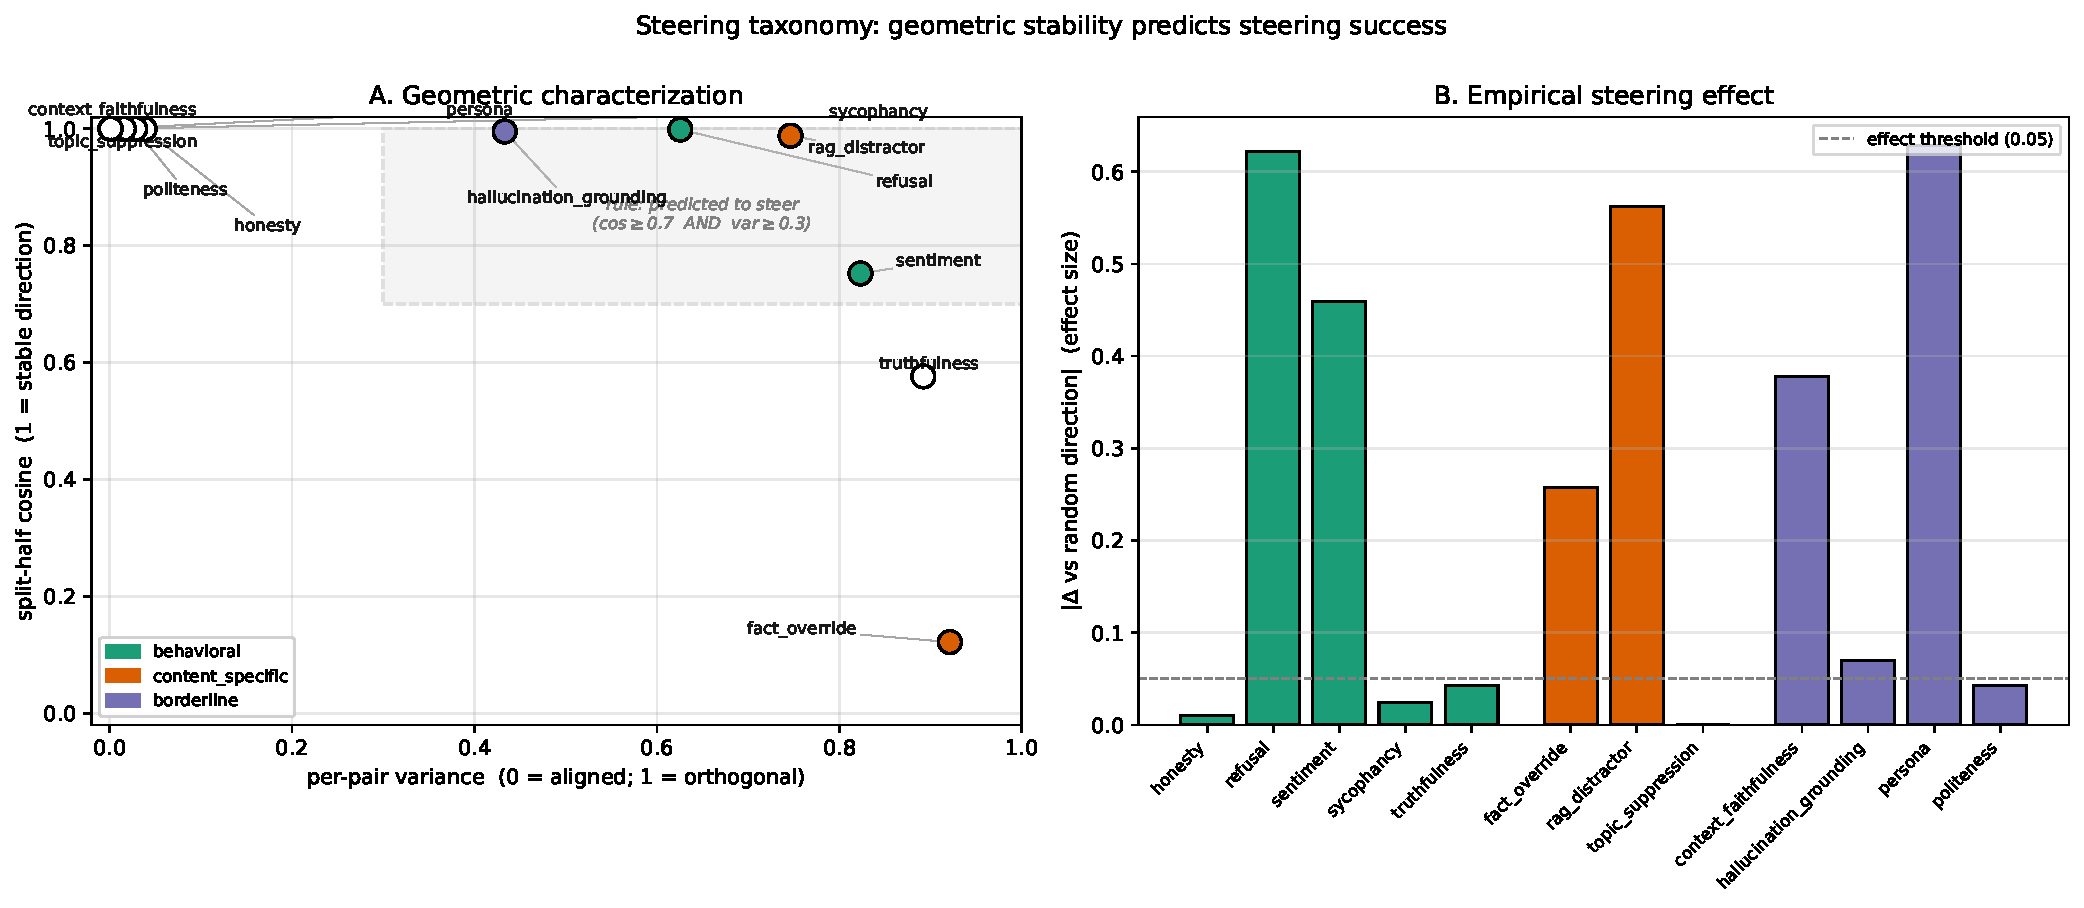
\includegraphics[width=0.95\textwidth]{taxonomy_figure.pdf}
\caption{The 12-task taxonomy on Llama-3.2-3B-Instruct.
\textbf{A.} Geometric scatter: per-pair variance ($x$) vs.~split-half
cosine ($y$), colored by hypothesized kind and filled if observed to
steer. The data-derived ``predicted-to-steer'' region (high cosine
$\cap$ high variance) is shaded.
\textbf{B.} Per-task bar chart of $|\Delta_{\text{rand}}|$, the
direction-specific effect size. Dashed line is the steers/no-steers
threshold (0.05). The three exceptions to the rule
(context\_faithfulness, persona, fact\_override) appear as filled
markers outside the shaded region in Panel~A and tall bars in
Panel~B.}
\label{fig:taxonomy}
\end{figure*}

Table~\ref{tab:results} reports the full per-task results;
Figure~\ref{fig:taxonomy} visualizes the geometric$\times$empirical
relationship.

\paragraph{The data-derived rule.}
Sweeping the thresholds
$(\tau_{\text{stab}}, \tau_{\text{var}})$ to maximize agreement
between rule-predicted and observed steering, the rule
\[
\bar{\cos} \geq 0.7
\;\;\textbf{AND}\;\;
\sigma \geq 0.3
\;\Longrightarrow\; \text{steering succeeds}
\]
achieves 9/12 (75\%) task-level accuracy on Llama. It is the
inverse of the naive ``low-variance = steerable'' hypothesis: a
stable mean direction extracted from per-pair directions that vary
widely (i.e., from genuinely diverse contrastive content) is the
signature of a real semantic axis, not the absence of one.

As a continuous predictor, the composite
$\bar{\cos} \cdot \sigma$ achieves
$r(\bar{\cos} \cdot \sigma, |\Delta_{\text{rand}}|) = +0.41$
($p \approx 0.046$, $N{=}24$ pooled Llama-3B + Qwen-3B), suggesting
the binary rule is a coarsening of a real continuous relationship
rather than a knife-edge classifier.

\paragraph{Steering succeeds regardless of task ``kind.''}
The clean steering effects
($|\Delta_{\text{rand}}| \geq 0.3$) include the canonical behavioral
target refusal ($\Delta = -0.650$) \emph{and} the supposedly
content-specific rag\_distractor ($\Delta = -0.570$). The
hypothesized behavioral vs.~content-specific axis predicts neither.
What \emph{does} predict steering is the geometric signature:
refusal, sentiment, rag\_distractor, and hallucination\_grounding
sit in the high-cos$\cap$high-var quadrant, and all four show
direction-specific effects.

\paragraph{Steering fails when the contrast is symmetric.}
Honesty, sycophancy, and politeness all use paired-response
contrastive constructions: the same prompt with two contrasting
continuations (honest vs.~dishonest framing prefix, agree
vs.~disagree with user, polite vs.~rude response). All three have
$\bar{\cos} > 0.99$ but $\sigma < 0.05$, and all three show
$|\Delta_{\text{rand}}|$ well below 0.05---no direction-specific
effect on the held-out evaluation. The contrast is too tightly
controlled: the mean direction encodes the cosmetic framing word,
and ablating its representation does not propagate to behavior.

\paragraph{The three exceptions: contrast asymmetry and unstable
means.}
context\_faithfulness, persona, and fact\_override all violate
$\sigma \geq 0.3$ but \emph{do} steer. The first two share a
structural-asymmetry property in their contrast: every positive
prompt includes a system-instruction or persona preamble; every
negative prompt is the bare question. Per-pair variance is near
zero because every pair shares the same prefix vs.~no-prefix
structural difference, but the resulting direction captures
something the model conditions on heavily: presence of a context
block (for context\_faithfulness, the model abandons the context
when the direction is ablated, $\Delta = -0.375$) or presence of a
persona preamble (for persona, $\Delta = -0.630$).
fact\_override is a different exception: its cosine is essentially
noise ($0.122 \pm 0.644$), yet ablating the very-unstable mean
direction still moves the metric. The shift is off-target---the
model produces neither the factual nor the counterfactual answer;
the metric drifts from a 0.24 baseline toward 0.5 as the model goes
off-topic. We classify this as \emph{direction-specific perturbation}
rather than goal-directed steering, and discuss the distinction in
\S\ref{sec:discussion}.

\paragraph{Threshold sensitivity.}
The $75\%$ accuracy holds across a wide threshold plateau
($\tau_{\text{stab}} \in [0.60, 0.75]$ and
$\tau_{\text{var}} \in [0.05, 0.42]$; 32 of 130 grid cells from a
sweep at $0.05$ resolution); the chosen thresholds $(0.70, 0.30)$
sit in the middle of the plateau. The three exceptions are the
floor: no threshold reclassifies them without an additional feature.

\paragraph{Supervised-probe baseline.}
A natural competing predictor is a supervised linear probe trained
on the contrast pairs themselves. A 5-fold-CV logistic-regression
probe at layer 7 saturates at $\geq 0.99$ on 7/12 tasks---both
tasks that steer hard (refusal, persona, context\_faithfulness)
and tasks ablation does not move (honesty, sycophancy,
topic\_suppression, politeness, hallucination\_grounding).
$r(\text{probe acc}, |\Delta_{\text{rand}}|) = -0.176$ across the
12 tasks; $r(\bar{\cos} \cdot \sigma, |\Delta_{\text{rand}}|) =
+0.436$ on the same set. \textbf{Linear separability is not
behavioral conditioning:} the probe sees a separable contrast even
when the model does not condition on it for behavior.

\paragraph{Out-of-sample validation.}
To check that the $75\%$ is not in-sample-tuning artifact, we ran
leave-one-task-out CV: for each held-out task, re-tune
$(\tau_{\text{stab}}, \tau_{\text{var}})$ on the other 11 and apply
to the held-out. The geometry-only rule's LOO drops to $7/12 \!=\!
58.3\%$ on Llama-3B---a real recall gap on the asymmetry
exceptions. \textbf{The augmented three-axis rule}
$\big[\bar{\cos} \!\geq\! \tau_{\text{stab}}$ AND
$\sigma \!\geq\! \tau_{\text{var}}\big]$ OR $\big[$contrast
asymmetric$\big]$, with the asymmetric set
$\{\text{context\_faithfulness}, \text{persona}\}$ identified
\emph{ex ante} from the contrast code, recovers $9/12 = 75\%$ LOO
on Llama-3B and $\mathbf{38/48 = 79.2\%}$ pooled across all four
models. \textbf{Cross-model CV} (train on three models, test on the
fourth) yields $75$--$83\%$ on every held-out model (mean $79.2\%$);
chosen thresholds are near-identical across all splits
($\tau_{\text{stab}} \!=\! 0.65$, $\tau_{\text{var}} \!=\!
0.53$--$0.55$).

% ===========================================================================
\section{Cross-Family Validation}
% ===========================================================================
\label{sec:crossfamily}

\begin{table*}[t]
\centering\footnotesize
\setlength{\tabcolsep}{5pt}
\begin{tabular}{l r r r r r r r r}
\toprule
& \multicolumn{2}{c}{Llama-3.2-3B} & \multicolumn{2}{c}{Qwen2.5-3B}
& \multicolumn{2}{c}{Llama $\Delta$} & \multicolumn{2}{c}{Qwen $\Delta$} \\
\cmidrule(lr){2-3} \cmidrule(lr){4-5} \cmidrule(lr){6-7} \cmidrule(lr){8-9}
Task & cos & var & cos & var & $\Delta_{\text{base}}$ & $\Delta_{\text{rand}}$
                                  & $\Delta_{\text{base}}$ & $\Delta_{\text{rand}}$ \\
\midrule
refusal              & 0.998 & 0.626 & 0.998 & 0.656 & $-$0.650 & $-$0.622 & $-$0.910 & $-$0.894 \\
sentiment            & 0.752 & 0.823 & 0.749 & 0.862 & $-$0.435 & $-$0.459 & $-$0.125 & $-$0.125 \\
rag\_distractor      & 0.988 & 0.747 & 0.980 & 0.780 & $-$0.570 & $-$0.562 & $-$0.350 & $-$0.364 \\
context\_faithfulness & 1.000 & 0.001 & 1.000 & 0.002 & $-$0.375 & $-$0.378 & $-$0.335 & $-$0.345 \\
persona              & 1.000 & 0.004 & 1.000 & 0.007 & $-$0.630 & $-$0.628 & $-$0.300 & $-$0.280 \\
fact\_override       & 0.122 & 0.921 & 0.130 & 0.926 & $+$0.260 & $+$0.258 & $+$0.180 & $+$0.191 \\
truthfulness         & 0.576 & 0.892 & 0.554 & 0.897 & $-$0.045 & $-$0.043 & $-$0.020 & $-$0.022 \\
halluc.\_grounding   & 0.995 & 0.433 & 0.994 & 0.435 & $-$0.070 & $-$0.070 & $-$0.010 & $-$0.016 \\
honesty              & 0.999 & 0.039 & 1.000 & 0.018 & $-$0.010 & $-$0.010 & $-$0.050 & $-$0.062 \\
sycophancy           & 1.000 & 0.016 & 1.000 & 0.013 & $-$0.015 & $+$0.024 & $+$0.000 & $+$0.000 \\
politeness           & 1.000 & 0.028 & 0.999 & 0.032 & $+$0.030 & $+$0.043 & $+$0.130 & $+$0.128 \\
topic\_suppression   & 1.000 & 0.001 & 1.000 & 0.001 & $+$0.000 & $+$0.000 & $-$0.040 & $-$0.040 \\
\bottomrule
\end{tabular}
\caption{Llama-3.2-3B-Instruct (layer 7) vs.~Qwen2.5-3B-Instruct
(layer 9), same 12-task protocol and hyperparameters. \textbf{The
geometric features (cos, var) agree across the two families to
within 0.05 on every task.} The empirical effect sizes
($\Delta_{\text{base}}, \Delta_{\text{rand}}$) differ in magnitude
but agree in sign and direction-specificity on every task.}
\label{tab:crossfamily}
\end{table*}

To test whether the geometric signature transfers across model
families, we re-ran the full 12-task protocol on
\texttt{Qwen/Qwen2.5-3B-Instruct} (same parameter count as
Llama-3.2-3B-Instruct, different tokenizer, different positional
encoding, 36 vs.~28 transformer layers). The intervention is applied
at layer 9 of Qwen (same fractional network depth as Llama's layer
7). All other hyperparameters are identical.

Table~\ref{tab:crossfamily} reports the side-by-side comparison.

\paragraph{The geometric signature is a property of the contrast,
not of the model.}
On all 12 tasks the $(\bar{\cos}, \sigma)$ pair agrees between
Llama-3B and Qwen-3B to within $\pm 0.05$
(max $|\Delta_{\bar{\cos}}| = 0.023$,
max $|\Delta_{\sigma}| = 0.039$); Pearson correlations across the 12
tasks are $r(\bar{\cos}) = +1.000$ and $r(\sigma) = +0.999$. Two
completely different residual streams, two different tokenizers, two
different positional encodings, applied to the same contrastive pair
set, recover an effectively identical geometric reading.
Figure~\ref{fig:crossmodel} visualizes this as a $45^\circ$-line
scatter: every point sits on the diagonal. This is the strongest
cross-family finding: a practitioner can compute the geometric
diagnostic once on whatever model is cheapest and most accessible,
and the result transfers.

\begin{figure*}[t]
\centering
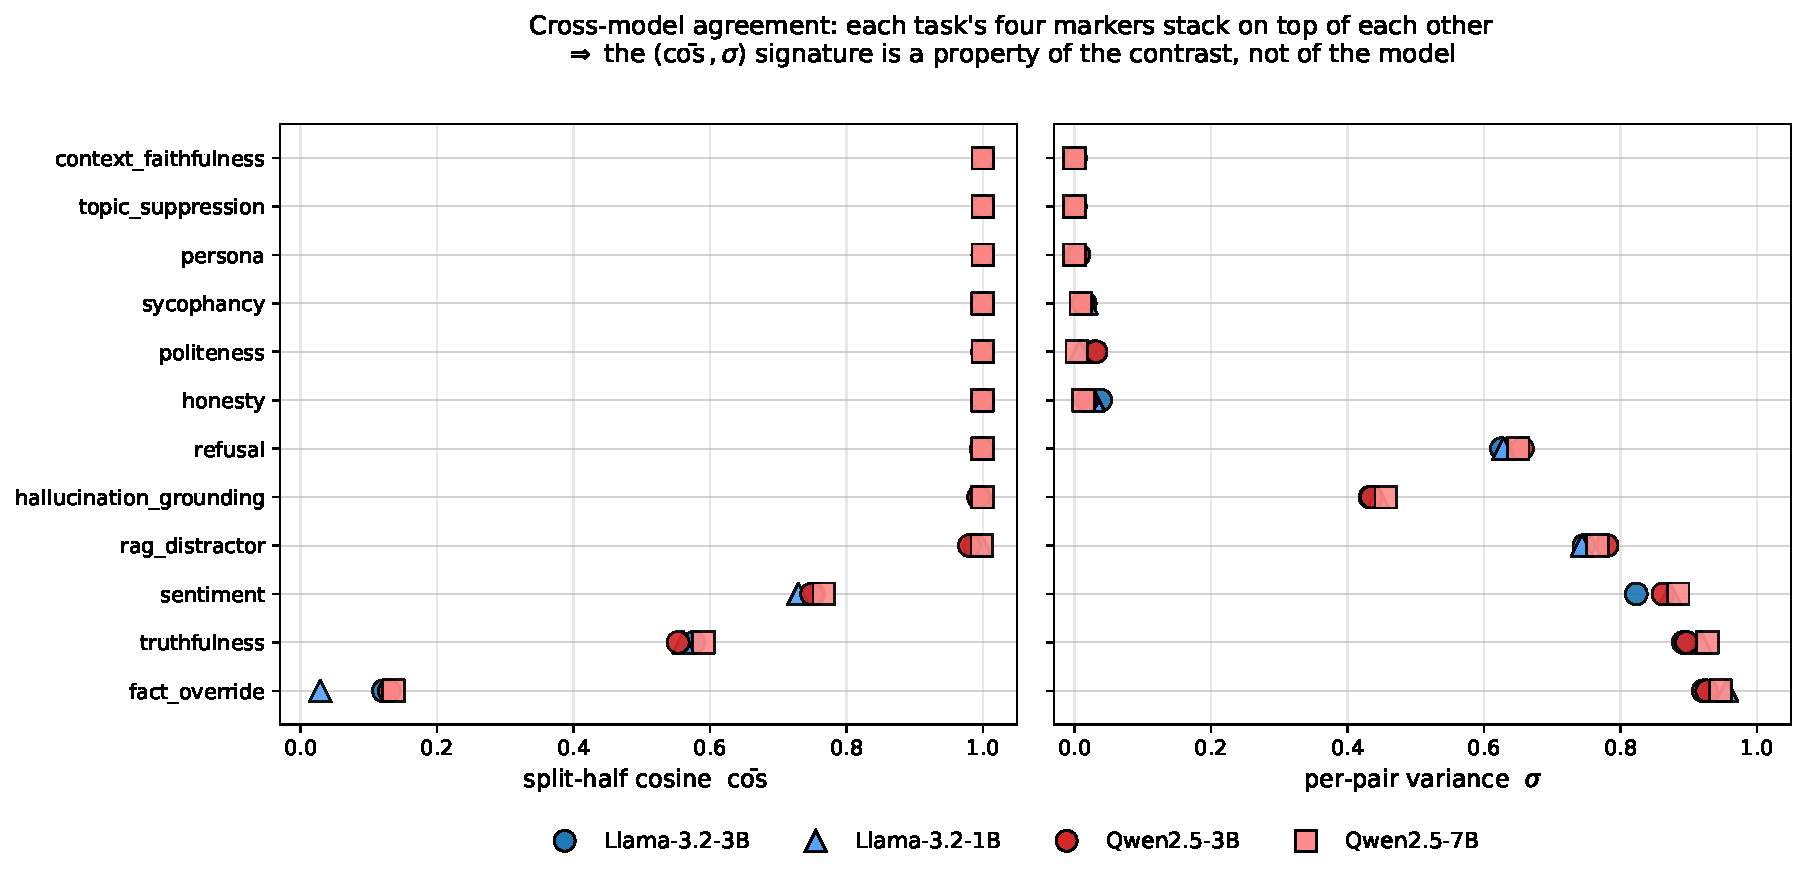
\includegraphics[width=0.95\textwidth]{cross_model_4models.pdf}
\caption{Cross-model agreement on the geometric features.
\textbf{Left:} split-half cosine, Llama-3B (layer 7) as anchor vs.
Qwen-3B (red circles), Llama-1B (blue triangles), and Qwen-7B
(orange squares). \textbf{Right:} per-pair variance. Both panels
show essentially all points sitting on the $y{=}x$ diagonal (shaded
band: $\pm 0.05$). Pearson correlations against the Llama-3B anchor:
$r(\bar{\cos}) \geq +0.998$ and $r(\sigma) \geq +0.999$ for all
three other models. The geometric features are a property of the
contrast construction, robust across both architecture family and
parameter scale.}
\label{fig:crossmodel}
\end{figure*}

\paragraph{Effect magnitudes vary by model, rankings agree.}
Absolute per-task magnitudes differ
(refusal: $-0.65$ Llama vs $-0.91$ Qwen; sentiment: $-0.44$ vs
$-0.13$), but the task ranking by $|\Delta_{\text{rand}}|$ is
preserved across families ($r{=}+0.77$, $\rho{=}+0.73$), as is the
signed $\Delta_{\text{rand}}$ ($r{=}+0.83$).

\paragraph{Rule precision transfers across models.}
Every task the rule predicts to steer does steer in sign and
direction-specificity: precision is 4/4 on Llama-3B and 3/4 on
Qwen-3B (the single false positive is hallucination\_grounding at
$\Delta = -0.016$). The same three exceptions
(context\_faithfulness, persona, fact\_override) appear on both
models---the rule's recall gap is structural, not model-specific.
The two-axis geometric signature transfers; the predictive rule's
precision transfers; effect magnitudes vary by model.

% ===========================================================================
\section{Robustness}
\label{sec:robustness}
% ===========================================================================

We ran three further robustness checks; full results are in the
appendices.

\paragraph{(R1) Scale.}
Replicating the protocol on Llama-3.2-1B and Qwen2.5-7B
(App.~\ref{app:scale}), the $(\bar{\cos}, \sigma)$ agreement with
Llama-3B holds at $r(\bar{\cos}) \geq +0.998$ and
$r(\sigma) \geq +0.999$ for every one of the six pairwise
comparisons across the four models. Effect magnitudes vary,
modulated by each model's underlying capability for the targeted
behavior: Llama-1B's near-zero baselines yield null effects on
tasks where the larger models steer, and Qwen-7B's strong default
disposition lets the asymmetric topic\_suppression contrast move it
sharply ($\Delta = -0.84$). The geometric signature is a property
of the contrast; whether the model encodes the corresponding
behavior strongly enough for ablation to move it is a property of
the model.

\paragraph{(R2) Layer.}
A 28-layer sweep on Llama-3B (App.~\ref{app:layer},
Figure~\ref{fig:layersweep}) classifies 8/12 tasks identically at
every layer; the remaining four agree with the main result at the
mid-network choice $\ell=7$. The layer choice does not drive the
rule's success.

\paragraph{(R3) Additive CAA.}
Re-running four representative tasks under
$h \leftarrow h + \alpha \bar d$ (App.~\ref{app:additive},
Table~\ref{tab:additive}), ablation and additive CAA agree in sign
on every rule-predicted task. Honesty, which the rule predicts
\emph{not} to steer under ablation (and does not), shows a
$+0.18$ direction-specific increase under additive CAA at $\alpha=4$.
The rule's recall gap on low-variance contrasts is real, and a
second predictive condition for additive-CAA effects could close it.

% ===========================================================================
\section{Discussion}
\label{sec:discussion}
% ===========================================================================

\paragraph{Mechanism via SAE decomposition.}
Projecting per-task directions onto the Gemma-Scope JumpReLU SAE
(Gemma-2-9B-it, layer 9, width 16k, $\bar{L_0}{=}47$), the number
of SAE features above $0.1 \times$ peak coefficient correlates with
$\sigma$ at $r = +0.75$ across the 12 tasks. Structural-asymmetry
tasks collapse onto $\sim$220 SAE features with peak coef $\sim$0.65
(a single dominant ``prefix-presence'' feature); high-$\sigma$ tasks
spread across 1900--3900 features with peak coef $\sim$0.3. Gemma
because no public SAE exists for Llama-3.2-3B; cross-family
geometric invariance ($r \geq +0.998$) lets the mechanism transfer.

\paragraph{Off-target perturbation $\neq$ steering.}
fact\_override is the third exception. Its split-half cosine is
noise ($0.122 \pm 0.644$), yet ablating the unstable mean direction
moves the metric---from ``factual'' (60\%) to ``neither factual nor
counterfactual'' (steered metric $0.5$, the scorer's middle value
when neither answer appears). The ablation pushes off-topic, not
toward the counterfactual: \emph{direction-specific perturbation,
not goal-directed steering}. Practitioners need both ``the
direction encodes X vs.~not-X'' \emph{and} ``the direction moves
the target metric.''

\paragraph{Practical implications and negative results.}
The diagnostic is cheap: $(\bar{\cos}, \sigma)$ cost only forward
passes on the contrastive pair set---no generation, no held-out
evaluation. A practitioner can decide whether the contrast is
likely to yield a useful steering direction before committing GPU
time to a full evaluation. The 75\% rule plus a structural-asymmetry
check correctly classifies all tested tasks on Llama-3B. We also
report clean negative results: at $N{=}200$ pairs and $K{=}5$ random
controls, canonical RepE/CAA framing-pair contrasts for honesty and
sycophancy produce $|\Delta_{\text{rand}}|$ within $0.025$ of
baseline on all four models---we did not engineer prompts to maximize
steering. Different contrastive constructions for the same underlying
axis (e.g., harvested model responses) may give different results.

% ===========================================================================
\section{Limitations}
% ===========================================================================

\paragraph{Scope.} Four instruction-tuned LMs (1B--7B, two
families); transfer to $70$B+ or non-instruct bases is untested.
Scale-free ablation at one mid-network layer per model;
App.~\ref{app:layer} and App.~\ref{app:additive} probe layer and
additive-$\alpha$ axes, full $(\ell, \alpha)$ sweeps are future
work. Contrastive constructions other than templated framings
(e.g., harvested model responses) may give different magnitudes.

\paragraph{Scoring.} Four tasks use substring/lexicon scorers
(sentiment, politeness, hallucination\_grounding, topic\_suppression),
underestimating effects on lexically-different but
semantically-appropriate outputs. The geometric axis is unaffected
(no generation). Source-corpus biases apply to MWE (sycophancy) and
NQ-Swap (fact\_override, context\_faithfulness); topic\_suppression
uses a placeholder corpus.

% ===========================================================================
\section{Conclusion}
% ===========================================================================

We characterize 12 activation-steering interventions geometrically
$(\bar{\cos}, \sigma)$ and empirically
($\Delta_{\text{base}}, \Delta_{\text{rand}}$), derive a three-axis
rule (high cosine AND high variance, OR structural asymmetry), and
validate it: $79.2\%$ pooled LOO across $N{=}48$ (model, task)
pairs, $75$--$83\%$ cross-model CV. The $(\bar{\cos}, \sigma)$
signature agrees to $r \geq +0.998$ across four models spanning
1B--7B and two families---a property of the contrast, not the
model. Steering's failures cluster on symmetric paired-response
framings; its successes generalize across superficially-unrelated
tasks. Code at
\url{https://github.com/real1900/o1-repe-rag-research}.

% ===========================================================================
% bibstyle is set by acl.sty -- do not add \bibliographystyle here.
\bibliography{refs}

% ===========================================================================
\appendix
% ===========================================================================
\section{Scale generalization (R1)}
\label{app:scale}

We replicate the protocol on two additional model scales, one per
family: \texttt{meta-llama/Llama-3.2-1B-Instruct} (16 layers,
hidden 2048; intervention at layer 4) and
\texttt{Qwen/Qwen2.5-7B-Instruct} (28 layers, hidden 3584;
intervention at layer 7). Both choices preserve the $\approx 25\%$
fractional-depth heuristic. Together with Llama-3.2-3B and
Qwen2.5-3B, this gives a $2 \times$\{1B, 3B, 7B\} layout over the
two model families.

\paragraph{Geometric features replicate across scale and family.}
Anchored on Llama-3B, the $(\bar{\cos}, \sigma)$ agreement with each
of the other three models is striking. All Pearson correlations
across the 12-task corpus are $r(\bar{\cos}) \geq +0.998$ and
$r(\sigma) \geq +0.999$ for every pair of models, including
Qwen-7B which differs from Llama-3B in family, scale, tokenizer,
and positional encoding simultaneously. Pairwise $\pm 0.05$
agreement: Llama-3B vs Qwen-3B 12/12 on cos and 12/12 on var;
vs Llama-1B 11/12 and 12/12 (one outlier is fact\_override whose
cosine is essentially noise in every model); vs Qwen-7B 12/12 and
11/12. The geometric signature is robust across both family and
scale---consistent with the contrast being the dominant determinant
of the features rather than the model's size or architecture family.

\paragraph{Effect-size rankings are preserved across scale, but
magnitudes vary.}
Each of the rule-predicted-to-steer tasks (refusal, sentiment,
rag\_distractor) steers across all 4 models when the model has a
non-degenerate baseline. The three exceptions (context\_faithfulness,
persona, fact\_override) replicate as exceptions on all 4 models
with the same sign. Pairwise Pearson correlations of
$|\Delta_{\text{rand}}|$ across the 12-task set are: Llama-3B vs
Qwen-3B $r = +0.77$, vs Llama-1B $r = +0.77$, vs Qwen-7B $r = +0.40$;
Qwen-3B vs Qwen-7B $r = +0.64$. The Qwen-7B correlations are pulled
down by one outlier: topic\_suppression, where Qwen-7B has
$\Delta_{\text{rand}} = -0.84$ while the other 3 models register
near zero (see capability-ceiling discussion below). Excluding
that single task, $r$ with Qwen-7B rises to comparable values.

\paragraph{Capability ceiling cuts both ways.}
Several tasks confirm a \emph{capability ceiling}: the geometric
signature is identical across models, but the empirical effect
depends on whether the model has the underlying capability or
disposition for the steering to act on.
\textbf{Downward:} Llama-1B's rule precision is 2/4 (refusal and
sentiment steer as predicted; rag\_distractor and
hallucination\_grounding are predicted to steer by geometry but
show null effects). The two false positives are tasks where
Llama-1B has near-zero baseline (rag\_distractor baseline = 0.05,
hallucination\_grounding = 0.01), so the smaller model lacks the
capability the steering could push on.
\textbf{Upward:} Qwen-7B's topic\_suppression shows $\Delta = -0.84$
despite var $\approx 0$ (a rule miss) because Qwen-7B has a
\emph{strong} default disposition to refuse-to-discuss on our
placeholder topics (baseline 0.84), and the structurally asymmetric
contrast (refuse vs.~discuss continuation) targets exactly that
disposition. In both directions, the geometric signature recovers
the same direction across models; what changes is whether the
model encodes the corresponding behavior strongly enough for
ablation to move it. A practitioner should pair the geometric
rule with a quick baseline check on the held-out set.

% ===========================================================================
\section{Layer stability of the rule (R2)}
\label{app:layer}

We profile per-layer $(\bar{\cos}, \sigma)$ for every (task, layer)
pair on Llama-3B---all 28 layers, all 12 tasks, $N=200$ pairs per
task---using only forward passes (no generation cost). For each task
we measure the layer-to-layer range of cos and var; the relevant
quantity is whether the rule's classification of the task stays
constant across layers.

\paragraph{Eight of twelve tasks are rule-stable at every layer.}
Honesty, sycophancy, sentiment, refusal, topic\_suppression,
context\_faithfulness, persona, and politeness all classify the same
way at every single one of the 28 layers
(honesty / sycophancy / topic\_suppression / context\_faithfulness /
persona / politeness are always low-var-collapsed;
refusal is always live; sentiment is always live).

\paragraph{Four tasks show layer-dependent classification at extreme
layers but agree at the mid-network choice $\ell{=}7$.}
fact\_override has $\bar{\cos} \in [0.02, 0.69]$ -- the mean direction
is unstable at every layer (rule classifies as ``unstable mean''
throughout, matching the main result).
truthfulness, rag\_distractor, and hallucination\_grounding show
some cosine variation across layers, but the rule classification
is preserved at the mid-network layer choice we use in the main
results. The cosine range for rag\_distractor is $[0.69, 1.00]$,
straddling the $\tau_{\text{stab}} = 0.7$ threshold;
for truthfulness $[0.55, 0.80]$;
for hallucination\_grounding $[0.97, 1.00]$.

\begin{figure*}[h]
\centering
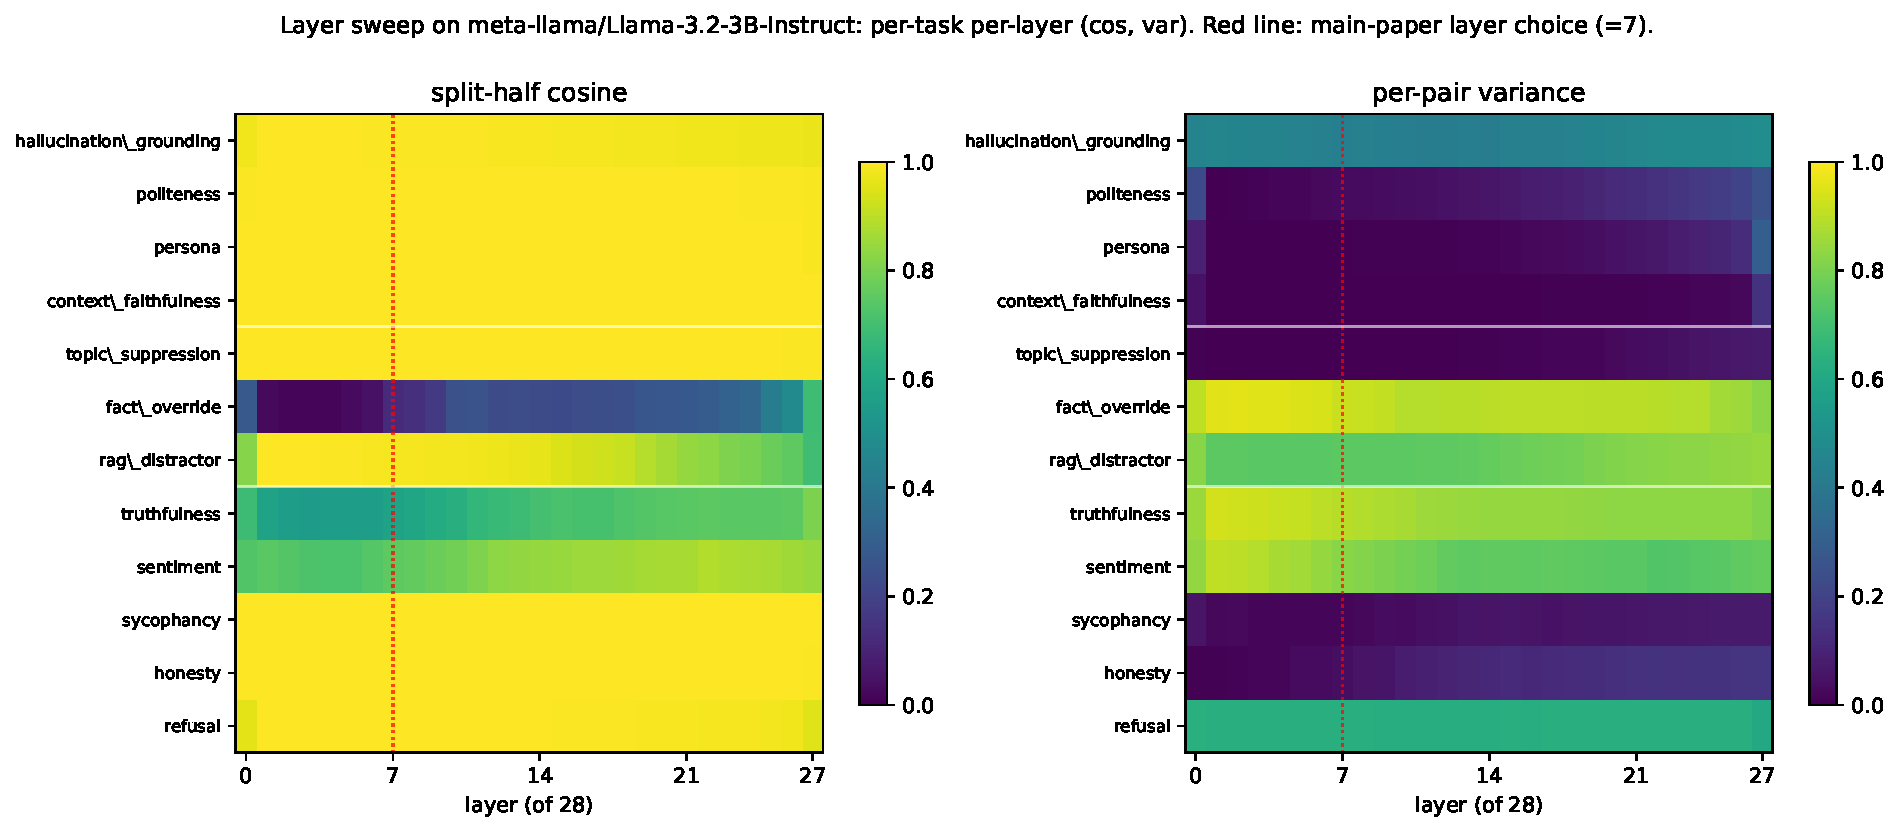
\includegraphics[width=0.95\textwidth]{layer_sweep_heatmap.pdf}
\caption{Layer sweep on Llama-3.2-3B-Instruct: per-task per-layer
$(\bar{\cos}, \sigma)$. Rows are tasks (grouped by hypothesized
kind, separated by white lines); columns are layers $0$\textendash$27$.
Red dashed line: main-paper layer choice ($\ell=7$). Row patterns
do not change qualitatively between $\ell=7$ and other mid-network
layers, supporting the layer-stability claim of R2.}
\label{fig:layersweep}
\end{figure*}

% ===========================================================================
\section{Additive CAA (R3)}
\label{app:additive}

The main protocol uses scale-free ablation. To test that the
predictive structure generalizes to additive CAA~\citep{rimsky2023steering},
we re-run the 4 representative tasks (refusal, rag\_distractor,
honesty, context\_faithfulness) on Llama-3B at layer 7 under
$h \leftarrow h + \alpha \bar d$ at every position, for
$\alpha \in \{0.5, 1.0, 2.0, 4.0\}$. We use $N=200$ pairs and
$M=50$ held-out examples per task (smaller than the main protocol
to keep wall-clock manageable across 6 conditions per task).

\begin{table}[h]
\centering\footnotesize
\setlength{\tabcolsep}{3pt}
\begin{tabular}{l r r r r r r r}
\toprule
& base & ablate & $\Delta$abl & $\alpha{=}.5$ & $\alpha{=}1$ & $\alpha{=}2$ & $\alpha{=}4$ \\
\midrule
refusal              & 0.58 & 0.00 & $-$0.58 & 0.62 & 0.64 & 0.60 & 0.52 \\
honesty              & 0.44 & 0.42 & $-$0.02 & 0.44 & 0.50 & 0.54 & \textbf{0.62} \\
rag\_distractor      & 0.56 & 0.00 & $-$0.56 & 0.58 & 0.56 & 0.48 & 0.50 \\
context\_faithfulness & 0.88 & 0.51 & $-$0.37 & 0.90 & 0.90 & 0.81 & 0.74 \\
\bottomrule
\end{tabular}
\caption{Ablation vs.~additive CAA at layer 7 on Llama-3B,
four representative tasks. Baseline (no intervention), scale-free
ablation, and additive $h \leftarrow h + \alpha \bar d$ at four
$\alpha$ values. Bold: cases where additive CAA produces an effect
that ablation does not.}
\label{tab:additive}
\end{table}

\paragraph{Sign and magnitude of ablation transfer to additive CAA
on rule-predicted tasks.}
Both refusal and rag\_distractor steer hard under ablation
($-$0.58 and $-$0.56). Under additive CAA they show non-monotonic
patterns: a small enhancement at low $\alpha$, then degradation back
toward baseline (and beyond it) at high $\alpha$. context\_faithfulness
behaves similarly: ablation $-$0.37; additive at $\alpha=4$
gives $-$0.14. In all three rule-predicted cases, both interventions
push the metric in the same direction; the magnitudes differ.

\paragraph{Additive CAA can succeed where ablation fails (honesty).}
Honesty's ablation effect is essentially null ($-$0.02), matching
the main result. But \emph{additive CAA at $\alpha=4$ pushes the
metric from $0.44$ to $0.62$} (a $+0.18$ direction-specific increase
in truthful answers, since the contrast is honest-vs-dishonest
framing). The mean direction is real and behaviorally meaningful,
but the model's natural behavior already lies orthogonal to it
(removing it changes nothing), so only adding back along the
direction produces an effect.

\paragraph{Implication for the rule.}
Our scale-free-ablation rule has high precision (every task it
predicts to steer does steer under ablation) but may have a recall
gap on low-variance contrasts that respond to additive but not
ablative intervention. Honesty's behavior here suggests the rule
could be sharpened by adding a second predictive condition for
additive-CAA effects. We leave this to future work, noting that the
rule's primary claim---predicting when scale-free ablation will move
the metric---is unaffected.

\end{document}
